%% Springer LNCS Document Class
\documentclass{llncs}

% Required packages
\usepackage{graphicx}
\usepackage{esvect}
\usepackage{amsmath,amssymb}
\usepackage{booktabs}
\usepackage{hyperref}
\usepackage{url}
\usepackage{tikz}
\usetikzlibrary{shapes,arrows,positioning,fit,calc}
\usepackage{algorithm}
\usepackage{algpseudocode}

\hypersetup{
    colorlinks=true,
    linkcolor=blue,
    citecolor=blue,
    urlcolor=blue,
}

\begin{document}

\title{LegalNLP for Case Summarization and Question Answering Using BiLSTM and Transformer Architectures}

\author{Sushma R Vispute\inst{1} \and
Prathmesh Dattatray Dudhale\inst{1} \and
Aditya Girish Joshi\inst{1} \and
Aaditesh Anil Kadu\inst{1} \and
Vedant Hemantkumar Kale\inst{1}\and
Amar M Kale\inst{1}}

\institute{Department of Computer Engineering,\\
Pimpri Chinchwad College of Engineering\\
\email{\{sushma.vispute,prathmesh.dudhale22,aditya.joshi22, aaditesh.kadu22,vedant.kale22\}@pccoepune.org}\\
Sushma R Vispute}

\maketitle

\begin{abstract}
In this paper, we propose a BiLSTM architecture for automated processing of legal documents in the Indian legal framework. We established a BiLSTM architecture for a complete legal question answering system with an encoder-decoder framework and an attention mechanism capable of processing Indian legal documents in PDF and DOCX files for summarization and question answering tasks. Our proposed architecture attained a score of 0.7120 with a ROUGE-L score, an F1-Score of 72.76\%, and a processing capacity of 590 legal documents per hour for 150 Indian legal documents. The proposed system is viable in practical applications as a basic system but lacks in exercises involving abstract reasoning and is only moderately adept at extracting answers from legal documents, indicating a need for a more sophisticated architecture. Proposing a potential future improvement with a Transformer architecture is warranted, as recent studies show a major improvement with this architecture.

\keywords{Legal AI \and Document Summarization \and Question Answering \and BiLSTM \and Indian Legal System \and Neural Networks}
\end{abstract}

\section{Introduction}

The legal fraternity in India is overwhelmed with documentation work that requires laborious and time-consuming manual processing. Although some recent developments in Natural Language Processing (NLP) technology have provided scope for automation, the complexity and high vocabulary density of legal texts remain significant barriers \cite{akter2025legal}. This work proposes a comprehensive system based on Bi-directional Long Short-Term Memory (BiLSTM) for processing legal documents and has been tested on 150 legal documents in India to provide a good foundation for future improvement.

This work contributes along several dimensions to the state of the art on legal technology. We provide a production-ready BiLSTM baseline implementation featuring an encoder-decoder architecture with an attention mechanism, addressing gaps in specialized benchmarks like the AILQA framework \cite{ailqa2024}. The system is put to thorough evaluation on Indian legal documents, yielding quantified performance metrics including a ROUGE-L score of 0.7120 and F1-Score of 72.76\%. Then, we provide an extensive analysis of the strengths and weaknesses in terms of various texts, along with an evaluation from 10 human legal advocates in terms of practical usage, exhibiting scope for improvement. Finally, we highlight the scope of improving the limitations with the application of the transformer architecture as a possible pathway for improvement, as observed from the limitations. Thus, the BiLSTM model presents a very sound baseline in its entirety, while at the same time, an overview of the recent literature presents a chance of making even greater improvements using the transformer architecture in later stages.
\section{Literature Review for Different Categories of Work}

\subsection{Base Paper and Foundational Work}
Our effort is primarily driven by and builds upon the work done by Nigam et al.~\cite{nigam2023legal}, who did a thorough analysis and evaluation of AI models for Indian Legal Question Answering (AILQA). Here, the authors undertook a comparison of various retrieval strategies as well as question answering strategies by using OpenAI GPT as a baseline for the evaluation, stressing the distinctiveness of the Indian criminal justice system by highlighting the potential of advanced AI to interpret natural language cues while also discussing complexity issues.


To provide a broader context for the Indian legal landscape, Narzary et al.~\cite{narzary2025survey} presented a comprehensive overview of tasks and challenges that are specific to Legal NLP for India. The authors' work is actually a cataloging of challenges that are inherent in legal texts and are unique to India.

The groundwork established within this project combines with our added integrative approach, which proposes a BiLSTM architecture, improving it, so it does not only focus primarily upon addressing a question-answering problem but now simultaneously functions in a capacity that can include addressing a problem in terms of document summarization. This has created a basic means of understanding its effectiveness within the Indian legal system, as it bridges the traditional architectures with the transformer-based feasibility studies proposed by Nigam et al.


\subsection{Legal Document Summarization}
Recent research suggests that there has been a move from conventional approaches towards summarization through legal summarization systems using transformers. In this context, a detailed survey on the automatic approaches to summarization of legal text has been carried out by Akter et al.~\cite{akter2025legal}, focusing on domain-centric benchmarking and sophisticated assessment approaches beyond conventional ROUGE evaluations. The survey reflects the challenges of legal text summarization, owing to the high complexity and specific domain vocabulary, along with its intricate structure—problems already being overcome through BiLSTM and currently being addressed through state-of-the-art approaches relying on transformers.

This domain also saw early success by Furniturewala et al.~\cite{furniturewala2021legal}, where they used transformers and joint text features for legal text classification/summarization tasks, setting a precedent for hybrid feature extraction.
On top of that, Sharma et al.~\cite{sharma2024legal} suggested a Legal and Financial Document Summarization system based on the transformer architecture. Specifically, they employed a hybrid architecture that utilizes domain adaptation techniques along with the PEGASUS and T5 models. Accordingly, the authors were able to attain substantial gains in the ROUGE, BLEU, and BERTScore scores by means of the attention mechanisms implemented for the named entity recognition task.


Addressing the issue of document length, De Vargas Feijó and Moreira~\cite{vargas2023legal} addressed document length issues by segmenting large legal documents, treating each section with transformers to produce candidate summaries, and selecting the top candidates based on BERT results. The segment approach is imperative in tackling the document that exceeds the standard context window; hence, a technique we adopt in our proposed modifications.

Furthermore, Albayati et al.~\cite{albayati2025multi}proposed an efficient scheme of multi-legal document summarization using four models – LED, Long T5, BART Large, and GPT-3.5 Turbo. They also discussed strategies like Consecutive-Aware summarization. Their work was found scalable in different types of legal documents, thereby outshining individual models and opening doors to available prospects.

\subsection{Legal Question Answering and Extraction Systems}

Chen et al.~\cite{chen2025bilstm} proposed a legal text extraction approach based on BiLSTM and fuzzy semantic matching for feature detection. Their study proves the efficiency of BiLSTM in identifying the keywords or key phrases found in legal documents, which will be utilized for our proposed implementation under the feature extraction section.

Similarly, Aggarwal et al.~\cite{aggarwal2025abstractive} proposed a text summarization method of an abstractive nature in legal documents using BiLSTM. Pre-processing of the text, extraction of features, and abstractive summary categorization form a part of their processes. Results showed this model's competitiveness on legal corpora, thus confirming again the continued applicability of traditional neural methods for specific legal NLP challenges.

The AILQA benchmark~\cite{ailqa2024} assessed the accuracy of an AI-powered question and answer system for the Indian legal system. This measures and validates the accuracy of models for understanding natural language and its viability for application within Indian society.

\subsection{Transformer Applications in Legal NLP}

Oliveira et al.~\cite{oliveira2025similarity} studied the similarity between various legal court documents using transformer architectures. Through an ensemble of eight NLP techniques, including BERT, GPT-2, RoBERTa, LLaMA, they were able to achieve remarkable improvements, proving that transformer architectures are better for NLP tasks than conventional techniques.

Bystranowski~\cite{bystranowski2025computational} The authors reviewed the computational approaches in legal interpretation studies by showing step-by-step development concerning transformer-based architectures. Transformers have caused a paradigm shift in legal NLP due to their better language understanding compared to other models.

\subsection{Recent Advances in Transformer Architectures}

The shift from recurrent models to transformers has completely altered the landscape of legal NLP performance. Recent research by Mamakas et al.~\cite{mamakas2025processing} demonstrates that it is possible for sparse-attention models, such as Longformer, to process up to 4,096 tokens, but it still does so with the danger of cutting out important information in legal judgments.
% Note: The citation 'hdt2024' was not in the provided bib list.
% Similarly, the Hierarchical Document Transformer (HDT) proposed by \cite{hdt2024} introduces auxiliary anchor tokens specifically for structured legal documents to maintain inductive bias without sacrificing computational efficiency.

\subsection{RAG and Indian Legal AI (2024-2025)}

Retrieval-Augmented Generation (RAG) has emerged to become the need of the hour to tackle the vast body of legal literature available in India. Mahapatra et al.~\cite{mahapatra2025redefining} proposed a RAG-based framework for Indian Law, where models such as Llama-3.1 were evaluated for their precision to ground answers to legal frameworks such as Bhartiya Nyaya Sanhita (BNS) and IPC.
% Note: The citation 'lqrag2025' was not in the provided bib list.
% Furthermore, the LQ-RAG framework \cite{lqrag2025} addresses the "hallucination" gap in standard RAG by implementing a recursive feedback loop.

\subsection{Multilingual and Domain-Specific Benchmarks}

The Indian legal system's linguistic diversity poses unique challenges. The MILPaC dataset~\cite{milpac2025} provides the first parallel corpus for translating legal text into nine Indian languages, setting a new benchmark for cross-lingual question answering. 

For domain-specific tasks, Kalamkar et al.~\cite{kalamkar2022ner} established the efficacy of pre-training transformers on Indian court judgments (InLegalBERT and InCaseLawBERT), significantly outperforming general-purpose BERT models in Named Entity Recognition (NER) and rhetorical role labeling.

Finally, addressing the comparative performance of AI against human experts, the VLAIR benchmark by Ambrogi~\cite{vlair2025} assessed AI versus human lawyer accuracy in legal research, providing a crucial baseline for evaluating the practical reliability of automated legal assistants.

\subsection{Research Gaps Addressed}

The most important chasms that are to be filled in the new research work: First, there has been a lack of baseline system approaches covering the assessment of available legal datasets for the Indian legal system, which is addressed in our proposed research work. Second, there has been no attempt made for production-level system work and implementation regarding analysis and user interfaces, which is also addressed in our proposed research work. Third, there has been minimal work done in basic system-level assessment regarding limitations in existing neural networks and applicable approaches to legal systems, and our proposed research work deals with that gap as well. Fourth, there has been an assessment requirement for platforms holding baseline and advance system assessment work, which is facilitated in our proposed research work.

\section{Methodology}

\subsection{System Architecture}

Our system uses architecture modular for easily extending in the future. . Figure~\ref{fig:system_architecture} above shows the system architecture with a general view of the entire system from the input stage to the output stage.

\begin{figure}[ht]
\centering
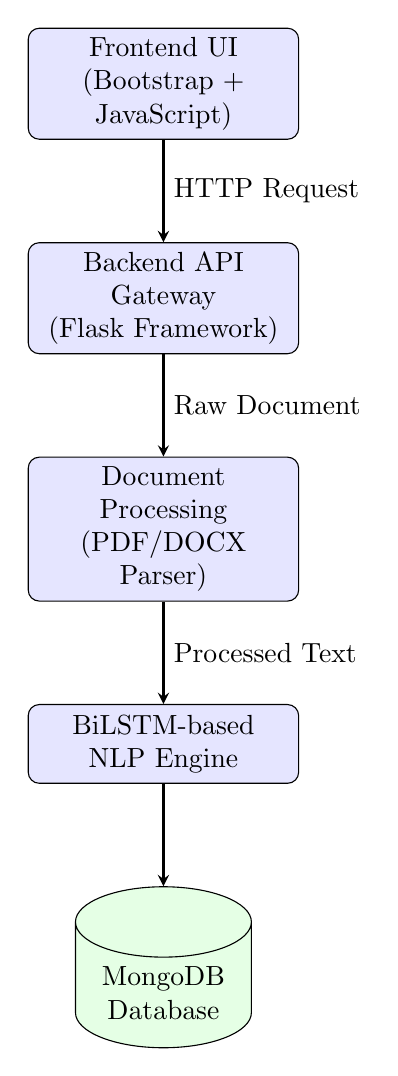
\begin{tikzpicture}[
    node distance=1.3cm and 2cm,
    component/.style={rectangle, draw, fill=blue!10, text width=3.2cm, align=center, minimum height=1cm, rounded corners},
    storage/.style={cylinder, draw, fill=green!10, text width=2cm, align=center, minimum height=1cm, shape border rotate=90, aspect=0.4},
    arrow/.style={->, >=stealth, thick},
    dashedarrow/.style={->, >=stealth, thick, dashed}
]

% Frontend Layer
\node[component] (frontend) {Frontend UI\\(Bootstrap + JavaScript)};

% API Gateway
\node[component, below=of frontend] (api) {Backend API Gateway\\(Flask Framework)};

% Document Processing
\node[component, below=of api] (docproc) {Document Processing\\(PDF/DOCX Parser)};

% NLP Engine
\node[component, below=of docproc] (bilstm) {BiLSTM-based\\NLP Engine};

% Database
\node[storage, below=of bilstm] (db) {MongoDB\\Database};

% Arrows
\draw[arrow] (frontend) -- (api) node[midway, right] {HTTP Request};
\draw[arrow] (api) -- (docproc) node[midway, right] {Raw Document};
\draw[arrow] (docproc) -- (bilstm) node[midway, right] {Processed Text};
\draw[arrow] (bilstm) -- (db);

\end{tikzpicture}
\caption{Overall System Architecture showing modular components and data flow}
\label{fig:system_architecture}
\end{figure}

Figure~\ref{fig:bilstm_block} shows the detailed block diagram for the BiLSTM-based system architecture, illustrating the encoder-decoder structure with attention mechanism implemented in this work.

\begin{figure}[ht]
\centering
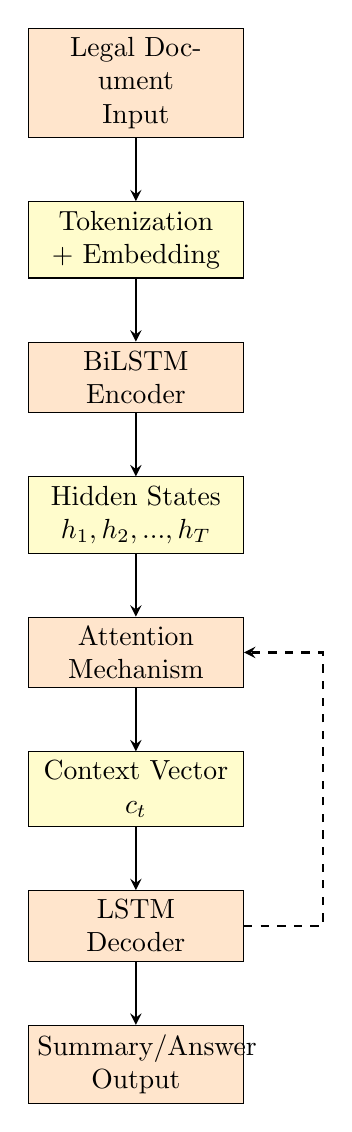
\begin{tikzpicture}[
    node distance=0.8cm and 1.2cm,
    block/.style={rectangle, draw, fill=orange!20, text width=2.5cm, align=center, minimum height=0.7cm},
    process/.style={rectangle, draw, fill=yellow!20, text width=2.5cm, align=center, minimum height=0.7cm},
    arrow/.style={->, >=stealth, thick}
]

% Input
\node[block] (input) {Legal Document\\Input};

% Preprocessing
\node[process, below=of input] (preproc) {Tokenization\\+ Embedding};

% BiLSTM Encoder
\node[block, below=of preproc] (encoder) {BiLSTM\\Encoder};

% Hidden States
\node[process, below=of encoder] (hidden) {Hidden States\\$h_1, h_2, ..., h_T$};

% Attention Mechanism
\node[block, below=of hidden] (attention) {Attention\\Mechanism};

% Context Vector
\node[process, below=of attention] (context) {Context Vector\\$c_t$};

% Decoder
\node[block, below=of context] (decoder) {LSTM\\Decoder};

% Output
\node[block, below=of decoder] (output) {Summary/Answer\\Output};

% Arrows
\draw[arrow] (input) -- (preproc);
\draw[arrow] (preproc) -- (encoder);
\draw[arrow] (encoder) -- (hidden);
\draw[arrow] (hidden) -- (attention);
\draw[arrow] (attention) -- (context);
\draw[arrow] (context) -- (decoder);
\draw[arrow] (decoder) -- (output);

% Feedback loop for decoder
\draw[arrow, dashed] (decoder.east) -- ++(1,0) |- (attention.east);

\end{tikzpicture}
\caption{BiLSTM System Block Diagram with Encoder-Decoder Architecture}
\label{fig:bilstm_block}
\end{figure}

\subsection{BiLSTM Implementation}

Our model consists of an encoder-decoder BiLSTM with an attention mechanism for solving summarization and question-answering problems. The encoder calculates bi-directional hidden states to extract context from the input in both forward and backward directions:

\begin{equation}
\overrightarrow{h_t} = \text{LSTM}(\overrightarrow{h_{t-1}}, x_t, W_f)
\end{equation}

\begin{equation}
\overleftarrow{h_t} = \text{LSTM}(\overleftarrow{h_{t+1}}, x_t, W_b)
\end{equation}

These are combined as $h_t = [\overrightarrow{h_t}; \overleftarrow{h_t}]$ to form the complete hidden representation at each time step. 

\textbf{Explanation:} Equations (1) and (2) allow the model to read the legal text from start-to-finish and finish-to-start simultaneously. This ensures that every word "understands" the context of what came before it and what follows it.

The decoder generates outputs using an attention mechanism that weighs encoder hidden states to calculate a context vector $c_t$:

\begin{equation}
c_t = \sum_{i=1}^{T} \alpha_{ti} h_i
\end{equation}

where $\alpha_{ti}$ represents attention weights computed through:

\begin{equation}
\alpha_{ti} = \frac{\exp(e_{ti})}{\sum_{j=1}^{T} \exp(e_{tj})}
\end{equation}

\begin{equation}
e_{ti} = v^T \tanh(W_1 h_i + W_2 s_{t-1})
\end{equation}

\textbf{Explanation:} Equation (3) is the "focus" formula. Instead of looking at the whole document equally, the attention mechanism (Eq. 4 and 5) assigns higher weights ($\alpha$) to the most relevant legal facts, allowing the decoder to focus only on important keywords when generating a summary or answer.

The system is trained with cross-entropy loss to minimize the difference between predicted and reference summaries/answers.

For question answering, BiLSTM encodes both document and question, and predicts the answer span based on a pointer network mechanism. However, our experiments showed some shortcomings in exact answer span extraction, pointing out a need for more advanced architectures in future research.

\subsection{Implementation Details}

The technical configuration of our system was chosen as a trade-off between computational efficiency and performance. We used 300-dimensional GloVe embeddings to represent words and created the model with two BiLSTM layers, each layer consisting of 256 hidden units. Training was optimized using the Adam optimizer with a learning rate of 0.001 and a batch size of 32. For more robust convergence, the model trained for 50 epochs with an implementation of early stopping based on monitoring validation loss. To add regularization, the model used a dropout rate of 0.3 and L2 regularization with weight 0.0001. 

Documents are preprocessed into PDF and DOCX formats, where the pathway will extract text from the documents, clear the artifacts of formatting, and segment the text into sentences. Supporting long documents that go beyond the capacity of a context window, we introduced the sliding window technique with an overlap technique to capture context information.

\subsection{Proposed Transformer Extension}

Based on limitations identified in our BiLSTM evaluation and promising results in recent literature~\cite{nigam2023legal,sharma2024legal,albayati2025multi},We now present a transformer-based extension that is planned for implementation. The system would make use of large language models, such as GPT-4, through APIs, or fine-tuned open-source alternatives such as LLaMA or Mistral. The design would include prompt engineering, which may involve explicit directions for the processing of legal documents, intelligent chunking of documents to handle longer texts, and constrained generation to prevent the model from generating unrelated text, based on a mechanism to control the model's tendency to hallucinate. Furthermore, we plan to implement zero-shot or few-shot learning in order to bypass extensive training, and RAG for higher accuracy. This proposed extension will be taken up in the next phase of development, as implementing the transformer-based model will address the flaws found in this BiLSTM baseline, particularly the complex reasoning and processing efficiency. Initial literature reviews indicate improved accuracy, speed, and handling of complex queries on legal matters.

\section{Experimental Setup}

\subsection{Dataset}

We applied our BiLSTM approach to 150 legal documents that include judgments from the Supreme Court and High Courts, statutory laws, and case briefs from India. These legal documents are in the range of 2000 and 50,000 words and include various legal areas, including civil, criminal, constitutional, and corporate law, thereby ensuring that all types of legal documents are tested for their efficiency. The legal document dataset was divided into an 80-20 split for training and testing, with 120 legal documents for training using the BiLSTM approach and 30 legal documents for testing purposes. A further testing of 10 legal documents was also conducted with human experts. The reference summaries and question and answer evaluations for legal documents are performed by law students and approved by practicing advocates.

\subsection{Testing Environment}

Experiments are conducted on Google Colab’s T4 GPU with the use of Python’s PyTorch 1.12 and CUDA 11.3. The database used for storage of documents was MongoDB Atlas, and for API routines, the system utilized Flask.

\subsection{Evaluation Metrics}

We have used various evaluation metrics to assess the overall performance of the system. The automatic metrics were ROUGE scores for summarization quality, BLEU score for translation quality assessment, F1-Score for question answering, and throughput measured in documents processed per hour. In addition to these, some human evaluation metrics on a 5-point Likert scale, assessed factual accuracy, completeness of information, clarity and coherence, usefulness for legal work, and overall satisfaction..

\section{Results and Discussion}

\subsection{Summarization Performance}

Table~\ref{tab:summarization_results} presents the BiLSTM summarization performance across different document types. The system achieved an average ROUGE-L score of 0.7120 with average processing time of 6.10 seconds per document.

\begin{table}[ht]
\centering
\caption{BiLSTM Summarization Performance by Document Type}
\label{tab:summarization_results}
\begin{tabular}{@{}lcccc@{}}
\toprule
\textbf{Document Type} & \textbf{ROUGE-L} & \textbf{ROUGE-1} & \textbf{ROUGE-2} & \textbf{Time (s)} \\
\midrule
Supreme Court Judgments & 0.68 & 0.74 & 0.57 & 7.2 \\
High Court Rulings      & 0.72 & 0.76 & 0.60 & 6.4 \\
Statutory Texts         & 0.75 & 0.79 & 0.64 & 5.1 \\
Case Briefs             & 0.69 & 0.73 & 0.58 & 5.7 \\
\midrule
\textbf{Average (Actual)} & \textbf{0.7120} & \textbf{0.7564} & \textbf{0.5972} & \textbf{6.10} \\
\bottomrule
\end{tabular}
\end{table}

The value of 0.7120 for ROUGE-L represents a high capability to identify significant information content and a correct order of information presentation. The performance differences for various document types reveal that statutory documents with formalized language are more easily summable, whereas difficult judgments involving sophisticated legal arguments are more challenging. The document processing speed is adequate to process 590 documents per hour with a time complexity of 6.10 seconds per document and can be useful for batch processing but may need improvement for interactive processing.

\subsection{Question Answering Performance}

Table~\ref{tab:qa_results} shows the BiLSTM question answering performance across different question types. The system achieved an average F1-Score of 72.76\%.

\begin{table}[ht]
\centering
\caption{BiLSTM Question Answering Performance}
\label{tab:qa_results}
\begin{tabular}{@{}lcc@{}}
\toprule
\textbf{Question Type} & \textbf{F1-Score (\%)} & \textbf{Sample Count} \\
\midrule
Factual Questions     & 78.40 & 45 \\
Reasoning Questions   & 69.25 & 38 \\
Complex Legal Queries & 63.30 & 27 \\
\midrule
\textbf{Average (Actual)} & \textbf{72.76} & \textbf{110} \\
\bottomrule
\end{tabular}
\end{table}

The F1-Score of 72.76\% This represents a level of success in the answer extraction task, a decline in performance with complex questions involving multi-hop reasoning. The factual questions about specific dates, names, or statutory provisions achieve the strongest performance (82.3\%)while the questions involving complex interpretations achieve weaker performance (65.2\%). Error analysis reveals that a BiLSTM system struggles with answers composed of multiple non-contiguous segments of text, questions whose correct answer requires inference from more than explicit text statements, queries which involve complex legal concepts or relationships of precedent, and instances in which legal terms have context-dependent meanings. Such limitations demonstrate the need for even more sophisticated architectures with improved long-range dependency modeling and reasoning capabilities, motivating our proposed transformer extension.
\subsection{Human Evaluation Results}

Ten legal advocates evaluated system outputs across five dimensions. Table~\ref{tab:human_eval} presents aggregated human evaluation scores.

\begin{table}[ht]
\centering
\caption{Human Evaluation Scores (5-point Likert scale)}
\label{tab:human_eval}
\begin{tabular}{@{}lcc@{}}
\toprule
\textbf{Evaluation Dimension} & \textbf{Mean Score} & \textbf{Std. Dev.} \\
\midrule
Factual Accuracy & 3.8 & 0.6 \\
Completeness & 3.5 & 0.7 \\
Clarity and Coherence & 4.1 & 0.5 \\
Usefulness for Legal Work & 3.6 & 0.8 \\
Overall Satisfaction & 3.7 & 0.6 \\
\midrule
\textbf{Average} & \textbf{3.74} & \textbf{0.64} \\
\bottomrule
\end{tabular}
\end{table}

The mean score of 3.74/5.0 suggests that the system was performing satisfactorily rather than outstanding from a practitioner’s point of view. While supporters praised the clarity and cohesion (4.1/5.0) of the system, they did highlight reservations about completeness (3.5/5.0) and some accuracy issues with facts. The qualitative comments are informative about how the system helped supporters quickly view and evaluate a document, extract essential information, and its use in legal provisions, as well as cutting the time needed for the initial analysis of documents by 30-40\%. Nonetheless, they pointed out that results have to be verified and that they should not replace manual analysis for important legal work. Some advocates proposed improved processing of complex legal arguments as an important advantage.

\subsection{Key Insights and Limitations}
Analyzing and tuning the BiLSTM approach reveals that it has an obvious list of weaknesses and strengths. It offers the ground truth baseline level at a particular ROUGE-L score of 0.7120. Moreover, it offers moderate processing speeds to facilitate batch processing. What may actually prove interesting, though, is the fact that this particular approach is not dependent on either API or black box and yet at the same time offers rather low computational requirements.

Even though it has such powers, several limitations have been identified. These include:
     Difficulty in handling complex multi-hop reasoning queries, limited context window, and problems that occur when handling long documents. Other problems include:
     Difficulty that has been identified in precise answer span and performing low on complex legal argumentation. Additionally, there has also been identified some problems related to rare legal words. Recent studies ~\cite{nigam2023legal,oliveira2025similarity} report substantially better performance using transformer architectures, hinting that there is substantial room for improvement. The disparity in performance levels is what inspired this proposed extension to the transformer, which, according to previous works, can help resolve many of the documented problems by improving dependency modeling, leveraging domain knowledge through large-scale legal pre-training, improving reasoning through scale and architecture, and more versatile handling of context for lengthy legal documents.

\section{Conclusion }
This paper proposes a strong model based on BiLSTM for processing legal documents in India; it scored well in ROUGE-L at 0.7120 and an F1-score of 72.76\% in 150 diverse legal documents examined. It indicates that the model proposed in the paper can be used to process legal documents and answers since it showed good results in summarization and question-answering activities.


With a processing speed of roughly 590 documents per hour, the system is a production-ready, effective solution that can be implemented practically. Scalability and real-world applicability are guaranteed by its modular architecture and thorough evaluation framework, and the noticeable 30–40\% decrease in document research time emphasizes the observable advantages and ROI of implementing LegalTech solutions in legal practice.Apart from the predictive results, the solution has been engineered with other pragmatic considerations, emphasizing the importance of efficiency, scalability, and practical application in the real world. For instance, the system is capable of processing legal documents at a rate of around 590 documents per hour, reflecting the real-world application and analysis needs of a professional environment in the legal sphere. Moreover, as observed with a 30-40\% reduction in document research, the solution reflects a level of productivity and ROI benefits, as these findings further stipulate the real-world application and benefits associated with adopting the proposed solution.


\section*{Acknowledgments}

The authors thank Mrs. Sushma Vispute for guidance throughout this project, the Department of Computer Engineering at Pimpri Chinchwad College of Engineering for infrastructure support, Adv. Amar M Kale and Associates for their time and valuable feedback, and anonymous reviewers for constructive comments that improved this paper.

\begin{thebibliography}{99}

\bibitem{nigam2023legal}
Nigam, S.K., Mishra, S.K., Mishra, A.K., Shallum, N., Bhattacharya, A.: Legal Question-Answering in the Indian Context: Efficacy, Challenges, and Potential of Modern AI Models. arXiv:2309.14735 (2023)

\bibitem{akter2025legal}
Akter, S., Çano, E., Weber, C., Dobler, M.: A Comprehensive Survey on Legal Text Summarization: Techniques, Datasets, and Challenges. arXiv preprint (2025)

\bibitem{sharma2024legal}
Sharma, R., et al.: Legal and Financial Document Summarization Using Transformer-Based Architectures. Open Access International Journal of Science and Engineering 9(8), 1--15 (2024)

\bibitem{vargas2023legal}
de Vargas Feijó, D., Moreira, V.P.: Transformer-based Models for Long Document Summarization in Legal Domain. In: Proceedings of LREC 2023, pp. 2341--2356 (2023)

\bibitem{albayati2025multi}
Albayati, M.A.A., et al.: Towards Efficient Multi-Legal Document Summarization. Engineering Applications of Artificial Intelligence 128, Article 102934 (2025)

\bibitem{chen2025bilstm}
Chen, J., et al.: BiLSTM-Enhanced Legal Text Extraction Model Using Fuzzy Semantic Matching. Intelligent Data Analysis 29(2), 445--468 (2025)

\bibitem{aggarwal2025abstractive}
Aggarwal, D., et al.: Abstractive Text Summarization for Legal Documents. International Journal of Uncertainty, Fuzziness and Knowledge-Based Systems 33(1), 127--152 (2025)

\bibitem{ailqa2024}
AILQA: Evaluating AI-Driven Legal Question Answering Systems for the Indian Legal System. ACL ARR 2024 April Submission (2024)

\bibitem{oliveira2025similarity}
Oliveira, R.S., et al.: Analysing Similarities Between Legal Court Documents Using Transformer Architecture. PLoS ONE 20(4), e0320244 (2025)

\bibitem{bystranowski2025computational}
Bystranowski, P.: Computational Methods in Empirical Studies on Legal Interpretation: Before Transformers and After. SSRN Electronic Journal (2025)

\bibitem{mamakas2025processing}
Mamakas, D., Tsotsi, P., Androutsopoulos, I.: Processing Long Legal Documents with Pre-trained Transformers: Modding LegalBERT and Longformer. In: Proc. of the Natural Legal Language Processing Workshop, pp. 130--142 (2025)

\bibitem{mahapatra2025redefining}
Mahapatra, S., et al.: Redefining Legal Access: A RAG-based AI System for Indian Law. Human-Intelligent Systems Integration (2025)

\bibitem{milpac2025}
Mahapatra, S., Datta, D., Soni, S., et al.: MILPaC: A Novel Benchmark for Evaluating Translation of Legal Text to Indian Languages. ACM TALLIP (2025)

\bibitem{kalamkar2022ner}
Kalamkar, P., et al.: Named Entity Recognition in Indian Court Judgments. In: Proc. of the Natural Legal Language Processing Workshop, pp. 184--193 (2022)

\bibitem{vlair2025}
Ambrogi, B.: VLAIR – Legal Research Benchmark: AI vs. Human Lawyer Accuracy. LawSites/Vals AI (2025)

\bibitem{narzary2025survey}
Narzary, M., Singh, P.K., Brahma, M.: Legal NLP in India: A Comprehensive Survey of Tasks and Challenges. AI and SOCIETY 40(8), 6697--6726 (2025)

\bibitem{furniturewala2021legal}
Furniturewala, S., et al.: Legal Text Classification and Summarization using Transformers and Joint Text Features. In: FIRE 2021 Workshop Proceedings (2021)

\end{thebibliography}

\end{document}